\documentclass[12pt]{article}
\usepackage[margin=1in]{geometry}
\usepackage{titling}
\usepackage[T1]{fontenc}
\usepackage{tabularx}
\usepackage{graphicx}
\usepackage{amsmath}

\pretitle{\begin{center}\Huge\bfseries}
\posttitle{\par\end{center}\vskip 0.5em}
\preauthor{\begin{center}\Large}
\postauthor{\end{center}}
\predate{\par\large\centering}
\postdate{\par}

\title{Języki formalne i Techniki Translacji \newline Zadanie Domowe}
\author{Jakub Musiał 268442}
\date{Październik 2023}

\begin{document}

\maketitle

\hspace{1cm}

\section*{Lista 1 - Zadanie 1}
    Podać deterministyczne automaty skończone (DFA) akceptujące następujące języki nad
    alfabetem ${0, 1}$:
    \begin{enumerate}
        \item zbiór wszystkich łańcuchów o zakończeniu 101;
        \item zbiór wszystkich łańcuchów zawierających trzy kolejne jedynki;
        \item zbiór wszystkich łańcuchów, w których każdy blok złożony z pięciu kolejnych symboli
        zawiera co najmniej dwa zera;
        \item zbiór wszystkich łańcuchów zaczynających się od 1, które interpretowane jako binarna
        reprezentacja liczby całkowitej są wielokrotnością 7;
        \item zbiór wszystkich łańcuchów, w których piąty symbol od końca jest zerem.
    \end{enumerate}

\newpage

\subsection*{1. Zbiór wszystkich łańcuchów o zakończeniu 101}
    Automatem akceptującym zadany język jest:
    \begin{center}
    \begin{math}
        M_1 = (\{q_0, q_1, q_2, q_3\}, \{0, 1\}, \delta_1, q_0, \{q_3\})
    \end{math}
    \end{center}

    \noindent Gdzie $q_i \equiv $ najdłuższy prefix wzorca '101', który znajduje się na końcu tekstu ma długość $i$,
    a funkcja przejść $\delta_1$ jest zdefiniowana w następujący sposób:

    \begin{table}[h!]
        \centering
        \begin{tabularx}{0.255\textwidth}{| c | c | c |}
            \hline
            $q$ & $\delta_1(q, 0)$ & $\delta_1(q, 1)$ \\
            \hline
            $q_0$ & $q_0$ & $q_1$ \\
            $q_1$ & $q_1$ & $q_2$ \\
            $q_2$ & $q_0$ & $q_3$ \\
            $q_3$ & $q_2$ & $q_1$ \\
            \hline
        \end{tabularx}
        \caption{Funkcja przejść $\delta_1$}
        \label{table:delta_1}
    \end{table}

    \noindent
    \begin{figure}[h]
        \centering
        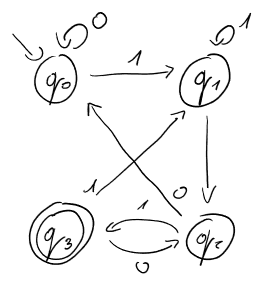
\includegraphics[width=0.5\linewidth]{img/m1.png}
        \caption{Schemat automatu $M_1$}
        \label{fig:m1}
    \end{figure}

\newpage

\subsection*{2. Zbiór wszystkich łańcuchów zawierających trzy kolejne jedynki}
    Automatem akceptującym zadany język jest
    \begin{center}
    \begin{math}
        M_2 = (\{q_0, q_1, q_2, q_3\}, \{0, 1\}, \delta_2, q_0, \{q_3\})
    \end{math}
    \end{center}

    \noindent Gdzie:
    \begin{itemize}
        \item $(\forall i \in \{0, 1, 2\})(q_i \equiv i \text{ ostatnich wczytanych liter z rzędu to } 1)$
        \item $q_3 \equiv \text{znaleziono (w dowolnym miejscu) ciąg co najmniej 3 jedynek}$
    \end{itemize}

    \noindent W automacie $M_2$ stan $q_3$ jest pochłaniający.
    \newline\newline
    Funkcja przejść $\delta_2$ dla tego automatu jest zdefiniowana w następujący sposób:

    \begin{table}[h!]
        \centering
        \begin{tabularx}{0.255\textwidth}{| c | c | c |}
            \hline
            $q$ & $\delta_2(q, 0)$ & $\delta_2(q, 1)$ \\
            \hline
            $q_0$ & $q_0$ & $q_1$ \\
            $q_1$ & $q_0$ & $q_2$ \\
            $q_2$ & $q_0$ & $q_3$ \\
            $q_3$ & $q_3$ & $q_3$ \\
            \hline
        \end{tabularx}
        \caption{Funkcja przejść $\delta_2$}
        \label{table:delta_2}
    \end{table}

    \begin{figure}[h]
        \centering
        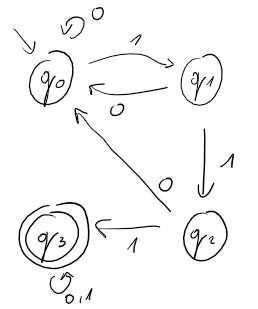
\includegraphics[width=0.5\linewidth]{img/m2.png}
        \caption{Schemat automatu $M_2$}
        \label{fig:m2}
    \end{figure}

\newpage

\subsection*{3. Zbiór wszystkich łańcuchów, w których każdy blok złożony z pięciu kolejnych symboli
zawiera co najmniej dwa zera}
    Automatem akceptującym zadany język jest
    \begin{center}
    \begin{math}
        M_3 = (Q_3, \{0, 1\}, \delta_3, q_\epsilon, F_3)
    \end{math}
    \end{center}

    \noindent Gdzie:
    \begin{itemize}
        \item $Q_3 = \{q_t\} \cup \{q_b : b \in \{0, 1\}^{\leq 5}\}$
        \item $\delta_3(q_t, l) = q_t$
        \item $|b| < 5 \implies \delta_3(q_b, l) = q_{(b|l)}$
        \item $
        |b| = 5 \implies \delta_3(q_b, l) =
        \begin{cases}
            q_{(b|l)[-5:]} & \text{: } c_0(b) \geq 2 \\
            q_t & \text{: w przeciwnym przypadku}
        \end{cases}$
        \item $F_3 = \{q_b : b \in \{0, 1\}^{\leq 4}\} \cup \{q_b : b \in \{0, 1\}^5 \land c_0(b) \geq 2\}$
    \end{itemize}

    \noindent \newline Oznaczenia:
    \begin{itemize}
        \item $q_t \equiv$ stan śmietnikowy
        \item $\{0, 1\}^{\leq n} \equiv$ ciągi bitowe o długości nie większej niż $n$ ($q_\epsilon \equiv$ ciąg bitowy o długości 0)
        \item $l \equiv$ litera alfabetu binarnego ($l \in \{0, 1\}$)
        \item $(b|l) \equiv$ konkatenacja ciągu $b$ i litery $l$
        \item $b[-n:] \equiv$ $n$ elementowy suffix ciągu  $b$ lub cały ciąg $b$, jeśli $|b| < 5$
        \item $c_0(b) \equiv$ liczba zer w ciągu $b$
    \end{itemize}

    \noindent \newline \textbf{Uzasadnienie poprawności:} \newline
    Stany automatu są indeksowane ciągami bitowymi o dlguości $\leq 5$ ($5$ ostatnich wczytanych bitów
    lub wszystkie wczytane bity, jeśli jest ich mniej niż $5$). Automat akceptuje wszystkie ciągi bitów o długości
    $< 5$ oraz te ciągi o długości $\geq 5$, w których każda piątka zawiera minimum $2$ zera. Wczytanie nowego bitu
    powoduje przejście do stanu powstałego poprzez dopisanie nowego bitu na koniec aktualnego ciągu indeksującego oraz -
    jeśli długość pamiętanego ciągu $= 5$ - usunięcie pierwszego pamiętanego bitu, gdy w pamiętamyn ciągu były minimum $2$ zera, lub
    do stanu śmietnikowego w przeciwnym przypadku (stan śmietnikowy jest pochłaniający, więc jeśli istnieje conjamniej
    jedna piątka w której nie ma odpowiedniej liczby zer, cały ciąg nie zostanie zaakceptowany).

    \newpage

    \begin{figure}[h]
        \centering
        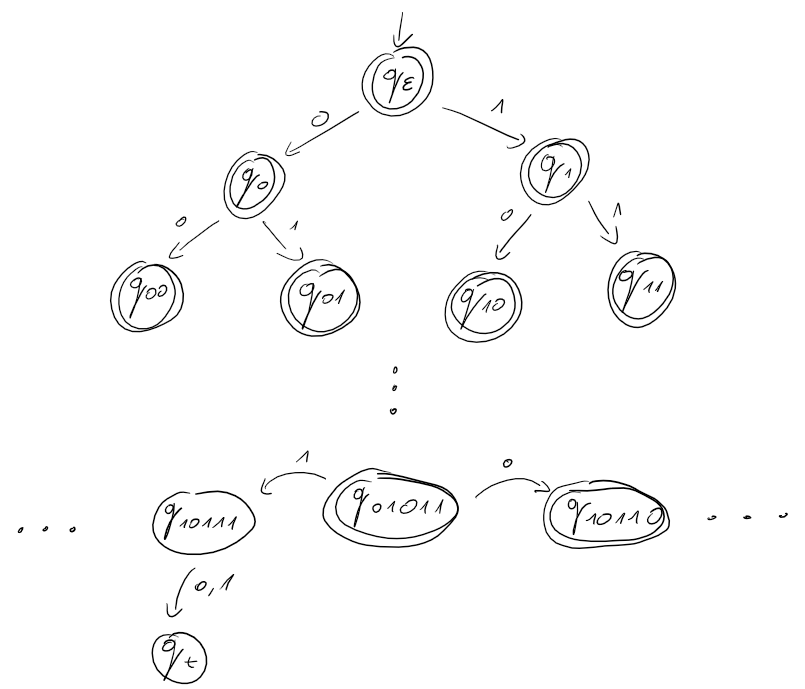
\includegraphics[width=\linewidth]{img/m3.png}
        \caption{Schemat automatu $M_3$}
        \label{fig:m3}
    \end{figure}

\newpage

\subsection*{4. zbiór wszystkich łańcuchów zaczynających się od 1, które interpretowane jako binarna
reprezentacja liczby całkowitej są wielokrotnością 7}
    Automatem akceptującym zadany język jest:
    \begin{center}
    \begin{math}
        M_4 = (\{q_t, q_\epsilon, q_0, q_1, ..., q_6\}, \{0, 1\}, \delta_4, q_\epsilon, \{q_0\})
    \end{math}
    \end{center}

    \noindent Gdzie:
    \begin{itemize}
        \item $q_t \equiv$ stan śmietnikowy
        \item $(\forall \: r \in \{0, ..., 6\})(q_r \equiv \text{reszta z dzielenia dotychczasowego ciągu przez } 7 \text{ jest równa } r)$
        \item $\delta_4(q_t, l) = q_t : l \in \{0, 1\}$
        \item $\delta_4(q_\epsilon, 0) = q_t \land \delta_4(q_\epsilon, 1) = q_1$
        \item $(\forall \: r \in \{0, ..., 6\})(\delta_4(q_r, 0) = q_{2r \text{ mod } 7} \land \delta_4(q_r, 1) = q_{(2r + 1) \text{ mod } 7})$
    \end{itemize}

    \noindent \newline \textbf{Uzasadnienie poprawności:} \newline
    Stany automatu są indeksowane resztami z dzielenia przez $7$ ($r \epsilon \{0, ..., 6\}$). Automat akceptuje
    wyłącznie stan $q_0$ - liczby podzielne przez $7$ (o reszcie z dzielenia przez $7$ równej $0$). Wczytanie kolejnego
    bitu $b$ jest równoznaczne z pomnożeniem liczby (reszty z dzielenia) przez $2$, jeśli $b = 0$, natomiast jeśli $b = 1$,
    jest to równoznaczne z pomnożeniem liczby przez $2$ oraz dodaniem $1$. Następnie z uzyskanej wartości ponownie należy wziąć
    resztę z dzielenia przez $7$, co daje indeks nowego stanu. Jeśli pierwszym wczytanym bitem jest $0$, automat przechodzi do
    pochłaniającego stanu śmietnikowego, więc automat akceptuje wyłącznie ciągi zaczynające się bitem $1$.

    \noindent
    \begin{figure}[h]
        \centering
        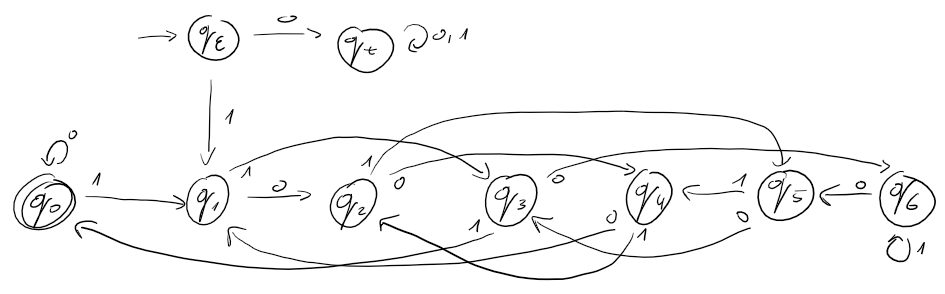
\includegraphics[width=\linewidth]{img/m4.png}
        \caption{Schemat automatu $M_4$}
        \label{fig:m4}
    \end{figure}

\newpage

\subsection*{5. Zbiór wszystkich łańcuchów, w których piąty symbol od końca jest zerem}
    Automatem akceptującym zadany język jest:
    \begin{center}
    \begin{math}
        M_5 = (\{q_{ijklm} : i, j, k, l, m \in {0, 1}\}, \{0, 1\}, \delta_5, q_{00000}, \{q_{0jklm} : j, k, l, m \in \{0, 1\}\})
    \end{math}
    \end{center}

    \noindent Gdzie:
    \begin{itemize}
        \item $q_{ijklm} \equiv$ 5 ostatnich wczytanych bitów to ciąg $(i, j, k, l, m)$
            (jeśli, liczba wczytanych bitów jest $< 5$, to ciąg ten uzupełniamy zerami od przodu)
        \item $\delta_5(q_{ijklm}, n) = q_{jklmn} : n \in \{0, 1\}$
    \end{itemize}

    \noindent \newline \textbf{Uzasadnienie poprawności:} \newline
    Stany automatu indeksowane są ciągami ostatnich $5$ wczytanych bitów. Zatem ze stanu $q_{ijklm}$
    po wczytaniu nowego bitu $n$ przechodzimy do stanu $q_{jklmn}$. Automat akceptuje stany postaci $q_{0jklm}$, zatem
    ciąg zostanie zaakceptowany, jeśli $5$-tym bitem od końca jest $0$. Automat akceptuje również wszystkie ciągi o
    długości $< 5$, ponieważ, jesli wczytaliśmy mniej niż $5 bitów$, to uzupełniamy ciąg zerami od przodu, by uzyckać
    $5$-biotwy indeks.


    \noindent
    \begin{figure}[h]
        \centering
        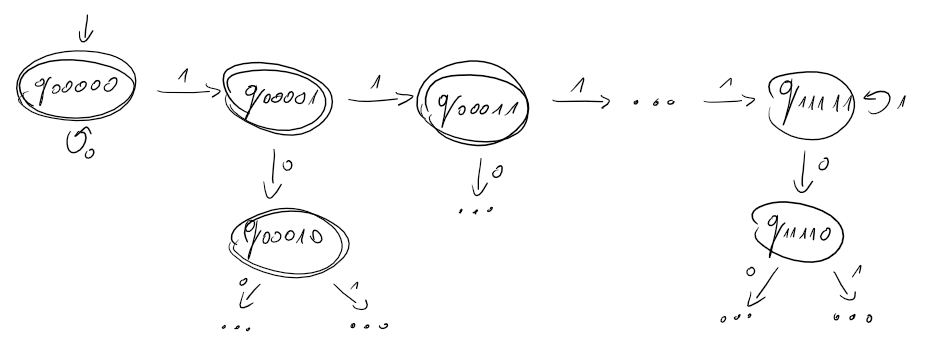
\includegraphics[width=\linewidth]{img/m5.png}
        \caption{Schemat automatu $M_5$}
        \label{fig:m5}
    \end{figure}

\end{document}
